Este capítulo tiene como objetivo definir las características principales que componen a los diferentes modelos y arquitecturas seleccionadas para el desarrollo de las dos tareas, las cuales surgen como ya se ha mencionado de la competición EXIST 2023. Por un lado, la primera de clasificación binaria de sexismo y la segunda de multiclasificación de la intención de los tweets clasificados como sexistas. Al tratarse de dos tareas similares se usarán para ambas los mismos modelos adaptados para clasificación binaria y clasificación multi clase.

Además, se incluirá un apartado para describir el entorno de trabajo, así como un para describir el preprocesamiento de los textos, fundamental para parte del estudio de este proyecto.

La implementación de las diferentes arquitecturas, así como diferentes procesos realizados durante el estudio se encuentran en el siguiente enlace: \href{https://github.com/ValenUC3M/-NLP-BachelorThesis-GonzaloValenti}{My Bachelor Thesis on NLP}.

Para cada uno de los modelos planteados a continuación el proceso de desarrollo es el mismo. En primer lugar, se definen los hiperparámetros, los cuales quedarán definidos junto a la descripción de cada modelo, así como para cada una de las diferentes versiones del dataset de lo cual se hablará más adelante. 

El entrenamiento se realiza cargando los diferentes modelos seleccionados a través de la librería HuggingFace \cite{HuggingFace}, una vez cargados los modelos, se evalúan las tareas con sus respectivas métricas para cada uno de los datasets de cada tarea.

Adicionalmente cabe destacar que durante este capítulo solo se hablarán tanto de los modelos base como de sus derivaciones a usar durante el trabajo. Esto es importante ya que por ejemplo dentro de la evaluación BERT también se evaluará con la variante multilingüe \cite{bert-base-multilingual-cased} o también por ejemplo roBERTa con una variante conocida como 'twitter-roberta-base-emotion'\cite{twitter-roberta-base-emotion,} de la cual se hablará más adelante.

A continuación se añade una tabla con los hiperparámetros usados para las diferentes pruebas. Cabe destacar que en este trabajo se han priorizado la experimentación de diferentes modelos respecto del ajuste fino de hiperparámetros por lo que, durante la fase de desarrollo, después de algunas pruebas, se llegó a la conclusión de que estos eran los mejores:

\begin{table}[H]
\begin{tabular}{|l|c|c|c|c|}
\hline
\rowcolor[HTML]{9B9B9B} 
{\color[HTML]{000000} \textbf{dataset}}              
& {\color[HTML]{000000} \textbf{batch size}} 
& {\color[HTML]{000000} \textbf{learning rate}} 
& {\color[HTML]{000000} \textbf{epochs}} 
& {\color[HTML]{000000} \textbf{weight decay}} 
\\ \hline
\rowcolor[HTML]{C0C0C0} 
\cellcolor[HTML]{9B9B9B}{\color[HTML]{000000} \textbf{Base}} 
& {\color[HTML]{000000} 16}               
& {\color[HTML]{000000} 2e-5}                  
& {\color[HTML]{000000} 3}             
& {\color[HTML]{000000} 0.01}                  
\\ \hline
\end{tabular}
\caption{Hiperparámetros usados durante la fase de generación de modelos.}
\end{table}


\section{Preprocesado} \label{preprocesado}

Durante el entrenamiento de los modelos se desea plantear dos alternativas para observar las mejorías que ofrece el preprocesamiento en materia de clasificación de tweets. Por un lado, se desea generar los modelos con el texto tal cual viene en el dataset y por el otro lado se desea observar si mejora o no los resultados realizar un preprocesamiento. Para ello primero se debe explicar el proceso que se desea seguir para realizar el preprocesamiento:

El objetivo del preprocesado es limpiar los tweets de toda aquella información que se considere que no aporta información e incluso puede generar ruido a la hora de entrenar. Para ello se ha realizado un breve estudio de preprocesado de tweets y se usa como referencia para ello tanto el estudio de 'tweet-sentiment-analysis-preprocessing' \cite{prepro1} como el trabajo de Abhishek Yadav llamado 'tweets-preprocessing' \cite{prepro2}.

Para realizar el preprocesado principalmente se han utilizado las siguientes librerías:
\begin{itemize}
                \item NLTK \cite{nltk} con el objetivo de eliminar todas las stop words tanto de los tweets en español como los de inglés.
                \item RE \cite{python_re} para generar expresiones regulares capaces de detectar y eliminar aquellas estructuras que se consideren innecesarias.
                \item Emoji \cite{python_emoji} con la cual elimina todos los emoticonos al tratarse de elementos no procesables por parte de los diferentes modelos basados en la arquitectura BERT.
            \end{itemize}


En primer lugar, se realiza un limpiado usando expresiones regulares de las menciones a usuarios al no ofrecer información de la frase y ser más un elemento propio de la red social. Además de las menciones se eliminan todos los hipervínculos, así como los hashtags por la misma lógica que con las menciones. No se desarrolla el proceso de borrado ya que se encuentra explicado de forma completa en el \href{https://github.com/ValenUC3M/-NLP-BachelorThesis-GonzaloValenti}{Github}.

Además del borrado de elementos propios de Twitter, también se eliminan los signos de puntuación, así como caracteres especiales y emojis. Al tratarse de elementos propios del lenguaje como las comas, puntos o paréntesis que no ofrecen realmente información de patrones de cara a los modelos se consideran innecesarios.

Lo último que se procesa de los tweets son las conocidas como 'stop words'. Son aquellas palabras vacías que carecen de significado si se usasen solas y que generalmente no son reconocidas por los diferentes algoritmos de NLP \cite{silva2003importance} ya que su objetivo es el de ofrecer coherencia y un efecto de naturalidad al lenguaje.


\section{Tokenización} \label{tokenización}

Además, los textos deben ser transformados en vectores de números reales para poder ser la entrada de los modelos transformadores que usamos en este trabajo. Este proceso comienza con la tokenización, que consiste en dividir el texto plano en subpartes llamadas tokens. El modelo preentrenado de un transformador proporciona un vector de números reales para cada uno de estos tokens.\cite{venkatesan2022implications}.

BERT utiliza lo que se llama un tokenizador WordPiece \cite{wordpiece}. Funciona dividiendo las palabras en sus formas completas (una palabra se convierte en un token) o en piezas de palabras, donde una palabra puede dividirse en múltiples tokens como se explica más adelante. Gracias a la tokenización se facilita la tarea de NLP al simplificar las palabras y eliminar elementos de ruido consiguiendo mejorar los resultados generales de las tareas \cite{webster1992tokenization}.

El uso de esta técnica permite a BERT representar palabras que no estaban presentes en la colección de textos utilizada para entrenar BERT, ya que generalmente compartirán algunos de los mismos tokens de entrada, que luego se alimentan en las primeras capas de BERT.

Por ejemplo, si cogiéramos la frase 'The embeddings are very useful for NLP' wordpiece generaría el siguiente resultado:

\begin{figure}[H]
    \centering
    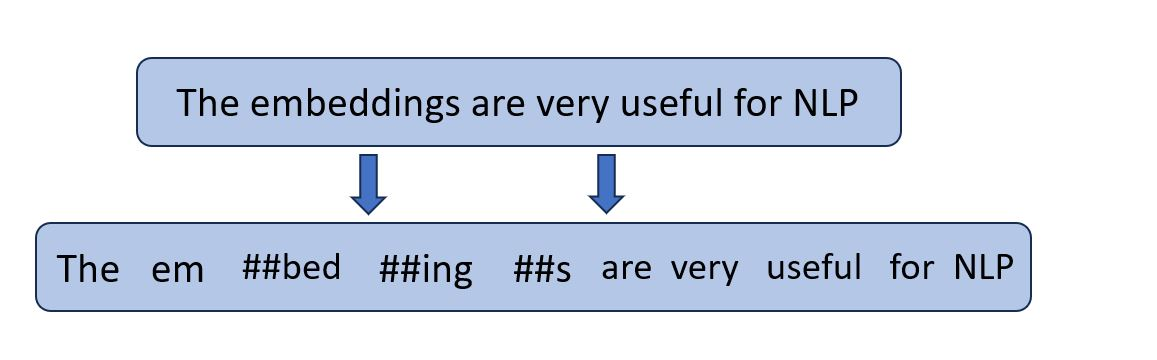
\includegraphics[width=12cm]{imagenes/Modelos/wordpiece.jpg}
    \caption{\centering Ejemplo de uso de Tokenización \cite{Bert-MLM}}
\end{figure}



\section{Modelos}
\subsection{BERT}
BERT o Bidirectional Enconder Representations from Transformers \cite{bert}, se considera el modelo base desde el que derivan los demás modelos de este trabajo. Es por eso que se realizará una explicación extensa sobre el mismo para entender adecuadamente su arquitectura y qué hace exactamente.

El objetivo de BERT \cite{devlin2018bert} es entender el lenguaje, es decir, aprender las diferentes relaciones que existen entre las palabras que componen un lenguaje. Si bien el modelo transformador original \cite{giacaglia2022transformers} estaba compuesto por un codificador y decodificador, BERT únicamente está formado por un codificador que transforma el texto de entrada en un conjunto de vectores (uno por cada token en el texto de entrada). 

En primer lugar, se explica el proceso de preentrenamiento del modelo BERT original. La colección de textos en Ingles usados para su entrenamiento se conoce como Toronto Book corpus \cite{toronto-book-corpus} y está compuesto de alrededor de 11.000 libros sin publicar de todo internet. Sin embargo, este dataset no existe en la actualidad, aunque existen intentos de recrearlo \cite{sgraaf-toronto}.

Para el uso de los Transformer se siguen dos estrategias principales: Por un lado, se realiza un proceso de enmascaramiento (MLM) y por otro lado un sistema de predicción de la siguiente oración (NSP). NSP (Next sentence prediction) es esencialmente un sistema de clasificación binaria que trata de predecir cuándo dos frases aparecen de forma consecutiva o no en un documento \cite{sun-etal-2022-nsp}. MLM (Masked Language Model) se define como un tipo de modelo de lenguaje que requiere ajuste fino para la mayoría de las tareas de procesamiento del lenguaje natural. Los MLMs se evalúan mediante sus puntajes de pseudo-verosimilitud, los cuales se calculan enmascarando tokens uno por uno. \cite{salazar2019masked}. De esta manera se puede predecir el token en cuestión y asignar diferentes pesos y valores a los diferentes tokens en base al entrenamiento realizado.

A continuación, se muestran los parámetros base predefinidos por el modelo sobre los que no se realizarán ajustes, para las diferentes arquitecturas BERT que se usarán durante el estudio de la tarea:

\begin{table}[H]
\begin{center}
\begin{tabular} {|c|c|c|c|c|}
\hline
\rowcolor[HTML]{C0C0C0} 
\textbf{Arquitectura}& \textbf{Capas} & \textbf{Nodos} & \textbf{Attention-Heads} & \textbf{Parámetros} \\ \hline
\cellcolor[HTML]{C0C0C0}\textbf{BERT-Base} & 12 & 768 & 12 & 110M \\ \hline
\cellcolor[HTML]{C0C0C0}\textbf{BERT-Large} & 24 & 1024 & 16 & 340M \\ \hline
\end{tabular}
\end{center}
\label{fig:bert-arch}
\caption{arquitecturas modelos Bert.}
\label{tab:arch-bert}
\end{table}


En primera instancia se debe entender correctamente el proceso de uso de BERT de cara a este trabajo. Una vez que el modelo ha sido preentrenado, y cuenta con una representación vectorial para cada palabra en función de su contexto, el modelo puede ser reentrenado para una tarea concreta ya sea clasificación de textos, análisis de sentimientos, reconocimiento de entidades, etc. A este proceso se le conoce como fine-Tunning. 

Debido a la gran cantidad de entrenamiento requerido y su elevado coste computacional, los modelos que se usan en este proyecto ya han sido preentrenados, y el esfuerzo de este proyecto se centra en el proceso de fine-Tunning. 

El aspecto técnico más innovador de BERT es el uso de aprendizaje bidireccional de Transformers usando mecanismos de atención, lo cual proporciona un contraste significativo respecto de sus anteriores predecesores que procesan de manera unidireccional pudiendo por ello entender el contexto de una palabra usando tanto sus predecesoras como antecesoras. De hecho, como ya se ha comentado, en contraposición con los modelos direccionales, BERT es capaz de leer la secuencia de palabras a la vez. Es por ello que realmente más que un modelo bidireccional, debería ser considerado un modelo no direccional por lo que es capaz de aprender el contexto de una palabra basándose en su entorno \cite{Bert-exp}.

La figura \ref{fig:bert-exp} muestra una descripción de alto nivel de la arquitectura de BERT (que consiste únicamente de un codificador). La entrada es una secuencia de tokens, donde cada palabra es inicializada con un embedding (vector). El codificador, basándose en las dos tareas MLM y NSP, será entrenado para producir una secuencia de embeddings (vectores), donde cada vector representa un token en la secuencia de entrada. 

\begin{figure}[H]
    \centering
    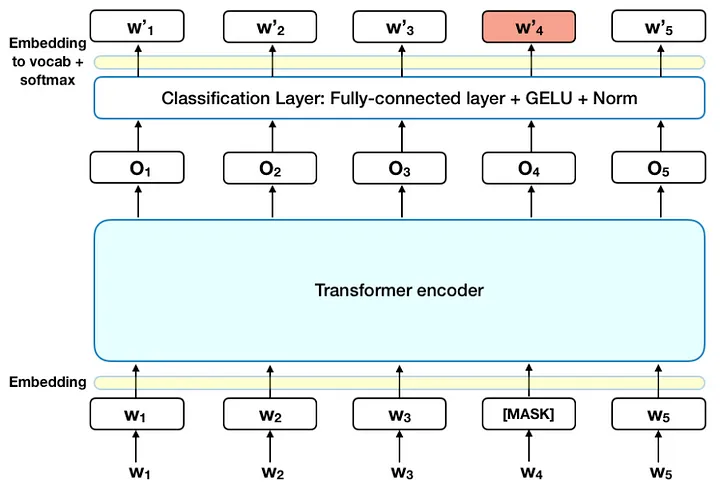
\includegraphics[width=10cm]{imagenes/Modelos/transformer-encoder.png}
    \caption{\centering Arquitectura de alto nivel del sistema transformer-encoder \cite{Bert-exp}}
    \label{fig:bert-exp}
\end{figure}


A continuación, para esta experimentación, se han utilizado dos versiones distintas de BERT: BERT-base-cased y BERT-base-uncased, cuya principal diferencia es que el primero distingue entre mayúsculas y minúsculas, mientras que el segundo no. 

%\section{BERT multilingüe}

BERT también proporciona un modelo multilingüe que fue entrenado con textos de 104 idiomas. Con la versión multilingüe, también experimentamos con las dos versiones: BERT-base-multilingual-cased \cite{bert-base-multilingual-cased} y BERT-base-multilingual-uncased \cite{bert-base-multilingual-uncased}

Sin embargo, durante el entrenamiento, como la mayoría de los textos estaban en inglés en comparación con otros idiomas, como el islandés que es escaso, los idiomas con menos datos fueron sobre muestreados usando técnicas de generación de textos y los idiomas con más datos fueron sub muestreados reduciendo su aparición en el proceso de entrenamiento \cite{pires2019multilingual}.

De cara a su arquitectura Y modelo, cabe aclarar que es la misma usada para bert ya mencionada en la \autoref{tab:arch-bert} mostrada durante la explicación de BERT. Por otro lado, el modelo elegido es el base al tener una limitación en el uso de la memoria para cargar el modelo large.


\subsection{RoBERTa}

Esencialmente RoBERTa es una extensión de BERT desarrollada con el objetivo de corregir algunos de los problemas detectados en BERT por \href{https://ai.facebook.com/research/}{Facebook AI Research (FAIR)}

RoBERTa está basado en BERT, aunque su tokenización es distinta, y está basada en Byte-Pair Encoding a nivel de byte como tokenizador como el que se usaba en GPT-2 \cite{GPT2}. Es decir, su tokenizador se asegura de que las palabras más frecuentes se representen usando un solo token mientras que las menos comunes se separan en tokens más pequeños, lo cual ha demostrado tener buenos rendimientos \cite{galle2019investigating}. 

Por otro lado, RoBERTa modifica el procedimiento de preentrenamiento de BERT entrenando el modelo durante más tiempo (1 Millón de pasos), con lotes más grandes (256 secuencias), sobre más datos (160GB de textos \cite{roberta-intro}) , eliminando el objetivo de predicción de la próxima oración y cambiando dinámicamente el patrón de enmascaramiento aplicado a los datos de entrenamiento, de tal manera que cada secuencia era enmascarada hasta 10 veces de manera diferente garantizando un proceso de aprendizaje más amplio y robusto respecto de BERT \cite{liu2019roberta}.

RoBERTa esencialmente mejora sus resultados respecto a BERT \cite{tarunesh2021trusting} en ciertas tareas considerando a RoBERTa como una versión más optimizada y robusta de BERT \cite{briskilal2022ensemble}. 

A continuación se muestran las variantes de roBERTa usadas:
\begin{enumerate}
    \item RoBERTa-base \cite{roberta-base}: De nuevo compuesta de la misma arquitectura que BERT-base descrita en la \autoref{tab:arch-bert}.
    \item Twitter-RoBERTa-base-emotion \cite{twitter-roberta-base-emotion}: Es una variante de RoBERTa que ha sido ajustada específicamente para el análisis de sentimientos en datos de Twitter. Ha sido entrenado en un conjunto de tweets (alrededor de 58M y está diseñado para identificar la polaridad de los tweets. Si bien a priori se podría considerar que no tiene interés para esta tarea, se ha considerado que al tratarse de una tarea donde se busca identificar el sexismo probablemente un modelo entrenado en sentimientos sea capaz de realizar aproximaciones precisas comparado con quizás la versión base del mismo twitter-roberta-base \cite{twitter-roberta-base}
\end{enumerate}

%\section{Modelo XLM-RoBERTa}
XLM-RoBERTa \cite{xlm-roberta} es una versión multilingüe del modelo RoBERTa, preentrenado en 2,5 TB de datos de CommonCrawl \cite{commoncrawl} que contienen 100 idiomas diferentes. 

Para entender bien XLM-RoBERTa se debe explicar primero el modelo XLM, el cual fue propuesto en el estudio Cross-lingual Language Model Pretraining \cite{lample2019cross} con el objetivo de aprovechar las similitudes y relaciones entre los diferentes idiomas para mejorar su capacidad de generalizar entre ellos.

Si bien XLM-RoBERTa es la versión de tanto XLM como RoBERTa, este no usa los datos de entrenamiento de XLM (como por ejemplo el corpus para francés, español, ruso, árabe y chino conocido como MultiUN \cite{ziemski2016united})  ni de RoBERTa, sino que como ya se ha mencionado usa sus propios datos.

Resumiendo, XLM-RoBERTa es una combinación de dos modelos poderosos: XLM, usando su idea de usar un preentrenamiento multilingüe y RoBERTa, del cual hereda su arquitectura y sistema de preentrenamiento. 

Esto permite que el modelo aprenda una representación bidireccional de la oración y extraiga características útiles desde una perspectiva multilingüe que se pueden utilizar para tareas en datasets multilingües.

A continuación, se muestran los dos modelos basados en XLM-RoBERTa, aunque el segundo modelo no se ha podido utilizar debido a una limitación de memoria en el hardware utilizado para el trabajo:
\begin{enumerate}
    \item XLM-roBERTa-base \cite{xlm-roberta-base}: Como ya se ha comentado posee la misma arquitectura que RoBERTa por lo que también la misma que BERT como se muestra en la \autoref{tab:arch-bert}.
    \item XLM-roBERTa-large \cite{xlm-roberta-large}: Se quería plantear el uso de XLM-Roberta large para ampliar la capacidad del modelo de generalizar y observar si se mejoran los resultados. Sin embargo, la plataforma en la que se realiza el trabajo tiene limitaciones que no cubren con la alta demanda de memoria del modelo ’large’, cuya arquitectura es la misma que para BERT-large mostrada en la \autoref{tab:arch-bert}. Por ello esa aproximación no se realizará y se incluirá en futuras mejoras.
\end{enumerate}


El proceso de estudio será equivalente para todos los modelos generados. Una vez seleccionado un modelo a estudiar se realizará cuatro iteraciones de ejecuciones usando para todas las mismas métricas de entrenamiento (factor de aprendizaje, batch size, épocas etc.) debido a un estudio previo para encontrar las mejores métricas bases para el estudio. 
Cada iteración realizará una de las siguientes combinaciones del dataset base:

\begin{itemize}
    \item Toda la colección de tweets, tanto en español como inglés, sin preprocesar.
    \item La colección de tweets en inglés
    \item Toda la colección de tweets, tanto en español como inglés, preprocesados usando la metodología ya explicada en \autoref{preprocesado}
    \item La colección de tweets en inglés
\end{itemize}

El objetivo de considerar diferentes colecciones para entrenar un modelo es estudiar qué efecto tiene el preprocesado sobre los resultados finales del modelo y, además, conocer qué ocurre si el corpus es entrenado con textos en ambos idiomas. 

\section{Entorno de trabajo}\label{entorno}
Esta sección tiene como objetivo explicar las diferentes herramientas utilizadas durante el desarrollo del trabajo:

    \begin{itemize}
        \item \href{https://colab.research.google.com/}{Google Collaboratory}: Google Collaboratory es una plataforma en línea gratuita que permite a los usuarios escribir y ejecutar código de Python en un entorno colaborativo en la nube. Proporciona acceso a recursos informáticos potentes y escalables, como GPU y TPU, lo que permite a los usuarios trabajar con grandes conjuntos de datos y realizar cálculos complejos de manera más eficiente.
        \item \href{https://code.visualstudio.com/Visual}{Studio Code}: Es un editor de código fuente desarrollado por Microsoft para Windows, Linux y macOS. Es una herramienta muy popular entre los desarrolladores de software, ya que es muy versátil y ofrece una amplia gama de características y extensiones para mejorar la productividad. 
        \item \href{https://www.google.com/intl/es_es/drive/}{Google Drive}: Es un servicio de almacenamiento en la nube gratuito ofrecido por Google que permite a los usuarios almacenar, compartir y sincronizar archivos en línea. También proporciona herramientas de productividad en línea para crear, editar y colaborar en documentos, hojas de cálculo y presentaciones.
        \item \href{https://github.com/}{GitHub}: Es una plataforma de desarrollo colaborativo de software basada en la web que utiliza el control de versiones Git para el seguimiento de cambios en el código fuente. Es una herramienta muy popular entre los desarrolladores de software, ya que permite a los usuarios colaborar en proyectos, contribuir al código y gestionar el flujo de trabajo de desarrollo de software.
        \item \href{https://www.overleaf.com/}{Overleaf}: Overleaf es una herramienta en línea para la edición y colaboración de documentos LaTeX, utilizada principalmente en la creación de documentos científicos y técnicos. Permite a los usuarios trabajar juntos en tiempo real en un solo documento, y proporciona herramientas para la edición, revisión y compilación de documentos LaTeX. En resumen, Overleaf es una herramienta en línea para la edición y colaboración de documentos LaTeX.
        \item \href{https://huggingface.co/}{El ecosistema Hugging Face}: Empezó como un repositorio de modelos Transformers y se ha convertido en un ecosistema para el desarrollo de modelos para NLP donde se pueden encontrar librerías específicas y herramientas para acelerar el uso e investigación en modelos Transformers \cite{tunstall2022natural}. HuggingFace proporciona esencialmente un acceso rápido y versátil a modelos Transformers para todo tipo de tareas y aproximaciones, es por ello que se usará como fuente de modelos durante el desarrollo de este trabajo.

    \end{itemize}
    
Hardware:

    \begin{itemize}
        \item Procesador: AMD Ryzen 5 3600 6-Core Processor 3.59 GHz.
        \item Tarjeta gráfica: Geforce GTX 1660.
        \item RAM: 16,0 GB.
        \item Sistema operativo: Windows 10 Home 64 bits.
    \end{itemize}
    

    
Los detalles del \textbf{Hardware} que ofrece Google Colab son los siguientes:

    \begin{itemize}
        \item Procesador: CPU Intel Xeon 2.20 GHz.
        \item GPU: Tesla K80.
        \item RAM: 13 GB.
        \item Sistema operativo: Linux.
    \end{itemize}